%%%%%%%%%%%%%%%%%%%%%%%%%%%%%%%%%%%
% PART I: User's manual
%%%%%%%%%%%%%%%%%%%%%%%%%%%%%%%%%%%

\part{User's manual}
\label{part:1}

\chapter{A short \GLOBES\ tour}
\label{chapter:tour}

To be written later: Short introduction such as ``With the following lines we obtain ...''
without detailed description of parameters. Should contain all most important functions of \GLOBES\ --
overview of main functions in \tabl{stdfunctions}.
Maybe: in form of long example which involves everything
and can be compiled.

\begin{table}[t]
\begin{center}
\begin{tabular}{p{3.8cm}p{3.8cm}p{7cm}}
\hline
Function & Purpose & Parameters \ra\ Result \\
\hline
\multicolumn{3}{l}{{\bf Systematics only:}} \\
\GLB{glbChiSys} & $\chi^2$ with systematics only  & ({\tt glb\_params in, int exp, int rule}) \ra\  {\tt double} $\chi^2$ \\[0.2cm]
\multicolumn{3}{l}{{\bf Projections onto axes:}} \\
\GLB{glbChiTheta} & Projection onto $\theta_{13}$-axis  &  ({\tt glb\_params in, glb\_params out, int exp}) \ra\  {\tt double} $\chi^2$ \\[0.1cm]
\GLB{glbChiDelta} & Projection onto $\deltacp$-axis  &  ({\tt glb\_params in, glb\_params out, int exp}) \ra\  {\tt double} $\chi^2$ \\[0.1cm]
\GLB{glbChiTheta23} & Projection onto $\theta_{23}$-axis  &  ({\tt glb\_params in, glb\_params out, int exp}) \ra\  {\tt double} $\chi^2$ \\[0.1cm]
\GLB{glbChiDm} & Projection onto $\ldm$-axis  &  ({\tt glb\_params in, glb\_params out, int exp}) \ra\  {\tt double} $\chi^2$ \\[0.1cm]
\GLB{glbChiDms} & Projection onto $\sdm$-axis  &  ({\tt glb\_params in, glb\_params out, int exp}) \ra\  {\tt double} $\chi^2$ \\[0.2cm]
\multicolumn{3}{l}{{\bf Projection onto plane:}} \\
\GLB{glbChiThetaDelta} & Projection onto $\theta_{13}$-$\deltacp$-plane  &  ({\tt glb\_params in, glb\_params out, int exp}) \ra\  {\tt double} $\chi^2$ \\[0.2cm]
\multicolumn{3}{l}{{\bf Projection onto any hyper-plane:}} \\
\GLB{glbChiNP} & Projection onto any $n$-dimensional hyper-plane  &  ({\tt glb\_params in, glb\_params out, int exp}) \ra\  {\tt double} $\chi^2$ \newline
Needs \GLB{glbSetProjection} before! \\[0.2cm]
\multicolumn{3}{l}{{\bf Localization of degeneracies:}} \\
\GLB{glbChiAll} & (Local) Minimization over all parameters  &  ({\tt glb\_params in, glb\_params out, int exp}) \ra\  {\tt double} $\chi^2$ \\
\hline
\end{tabular}
\end{center}
\caption{\label{tab:stdfunctions} \index{Standard functions (table)} The \GLOBES\ standard function to obtain a $\chi^2$-value with systematics only or systematics and correlations. The parameters {\tt rule} and {\tt exp}
can either be \GLB{GLB\_ALL} for all initialized experiment or the
experiment number ($0$ to \GLB{glb\_num\_of\_exps}-1) for a specific experiment. The format of \GLB{glb\_params} is discussed in detail in \Chapt~\ref{chapt:gettingstarted}. Note that all functions but {\tt ChiSys}
  are using minimizers which have to be initialized with \GLB{glbSetInputErrors} and \GLB{glbSetStartingValues} first.}
\end{table}

\chapter{Getting started with \GLOBES }
\label{chapt:gettingstarted}

In this first chapter of the user's manual, we assume that the \GLOBES\ software is readily installed on your computer system. For the installation,
see \App~\ref{app:installation} and the {\tt INSTALL} file in the
software package. We demonstrate how to load pre-defined experiments 
and re-obtain important information about them. In addition, we discuss
some standard concepts of the \GLOBES\ user interface. We do not go
into details of the programming language, which means that standard parts
of the program code common to all examples are, in general, omitted.
An example of a minimal \GLOBES\ program in C can be found on page~\pageref{ex:c}. Furthermore, the files of the examples in this part can be found in the {\tt Example} subdirectory of your \GLOBES\ distribution. \index{Examples} Since it depends on your installed
configuration, we refer to the {\tt README} file in the \GLOBES\ main directory, and the comments in the Makefile of the {\tt Example} subdirectory for how to complile the example files.

\example{Using \GLOBES\ with C}{\label{ex:c}
\index{C-Code}
Here comes the C-code sceleton, which is
(more or less) common to all of our \GLOBES\ examples:
\begin{quote}
{\tt {\footnotesize
\#include <stdio.h> \\
\#include <stdlib.h> \\
\#include <math.h> \\
\#include <string.h> \\
\\
\#include <globes/globes.h> \hspace*{0.5cm} /* Include GLoBES library */ \\
\\
\#include "myio.h" \hspace*{0.5cm} /* Include "housemade" I/O-routines */ \\
\\
/* If filename given, write to file; if empty, to screen: */ \\
char MYFILE[]="testX.dat"; \\
\\
int main(int argc, char *argv[]) \\
\{  \\
\\
 \hspace*{0.5cm} glbInit(argv[0]); \hspace*{0.5cm} /* Initialize GLoBES library */ \\
\\  
  \hspace*{0.5cm} glbInitExperiment("NuFact.glb",\&glb\_experiment\_list[0], \\
  \hspace*{1cm} \&glb\_num\_of\_exps); \hspace*{0.5cm} /* Initialize experiment NuFact.glb */\\
\\  
  \hspace*{0.5cm}  /* Initialize housemade output function */\\
  \hspace*{0.5cm} 
   InitOutput(MYFILE,"Format: ... ... ... $\backslash$n"); \\
\\  
  \hspace*{0.5cm} /* Initialize parameter vector(s) */ \\
  \hspace*{0.5cm} glb\_params true\_values = glbAllocParams(); \\
  \hspace*{0.5cm} /* ... */ \\
\\  
 \hspace*{0.5cm} /* Assign: theta12,theta13,theta23,deltacp,dm2solar,dm2atm */ \\
   \hspace*{0.5cm}  
     glbDefineParams(true\_values,\\
     \hspace*{1.5cm}asin(sqrt(0.8))/2,asin(sqrt(0.001))/2,M\_PI/4,M\_PI/2,7e-5,2e-3); \\
     
     \hspace*{0.5cm}  
   /* The simulated data are computed */ \\
   \hspace*{0.5cm} glbSetOscillationParameters(true\_values); \\
   \hspace*{0.5cm} glbSetRates(); \\
   
  \hspace*{0.5cm} /* ... CODE ... */ \\
  
\hspace*{0.5cm}  /* Destroy parameter vector(s) */ \\
\hspace*{0.5cm}  glbFreeParams(true\_values); \\
\hspace*{0.5cm} /* ... */ \\
 
  \hspace*{0.5cm}   exit(0); \\
\} 
}}
\end{quote}

}


\begin{table}[t]
\begin{center}
\begin{tabular}{llp{7cm}c}
\hline
Experiment & Filename & Short description & Refs. \\
\hline 
\multicolumn{3}{l}{\underline{Conventional beams:}} \\
??? & & \\[0.1cm]

\multicolumn{3}{l}{\underline{First-generation superbeams:}} \\
\JHFSK\ ($\nu$) & {\tt JHFSK.exp} & JHF (J-PARC) to Super-Kamiokande, neutrino running &  \cite{Huber:2002mx,Huber:2002rs} \\
\JHFSK\ ($\bar\nu$)& {\tt JHFSKanti.exp} & JHF (J-PARC) to Super-Kamiokande, antineutrino running &  \cite{Huber:2002rs} \\
\NUMI\  ($\nu$), OA $9 \, \mathrm{km}$ & {\tt NUMI9.exp} & NuMI with off-axis angle of $9 \, \mathrm{km}$ for $L=712 \, \mathrm{km}$, neutrino running & \cite{Huber:2002rs} \\
\NUMI\  ($\bar{\nu}$), OA $9 \, \mathrm{km}$ & {\tt NUMI9anti.exp} & NuMI with off-axis angle of $9 \, \mathrm{km}$ for $L=712 \, \mathrm{km}$, antineutrino running & \cite{Huber:2002rs} \\
\NUMI\  ($\nu$), OA $12 \, \mathrm{km}$ & {\tt NUMI12.exp} & NuMI with off-axis angle of $12 \, \mathrm{km}$ for $L=712 \, \mathrm{km}$, neutrino running & \cite{Huber:2002rs} \\
\NUMI\  ($\bar{\nu}$), OA $12 \, \mathrm{km}$ & {\tt NUMI12anti.exp} & NuMI with off-axis angle of $12 \, \mathrm{km}$ for $L=712 \, \mathrm{km}$, antineutrino running & \cite{Huber:2002rs} \\
\SPL\  ($\nu$) & {\tt SPL.exp} & SPL (CERN), neutrino running &  ??? \\
\SPL\  ($\bar\nu$) & {\tt SPLanti.exp} & SPL (CERN), antineutrino running & ??? \\[0.1cm]
 
\multicolumn{3}{l}{\underline{Superbeam upgrades:}} \\
\JHFHK\ ($\nu$) & {\tt JHFHK.exp} & JHF (J-PARC) to Hyper-Kamiokande superbeam upgrade, neutrino running &  \cite{Huber:2002mx,Huber:2002rs} \\
\JHFHK\ ($\bar\nu$)& {\tt JHFHKanti.exp} & JHF (J-PARC) to Hyper-Kamiokande superbeam upgrade, antineutrino running &  \cite{Huber:2002mx,Huber:2002rs} \\[0.1cm]

\multicolumn{3}{l}{\underline{Neutrino factories:}} \\
\NuFactI\ & {\tt NuFact.exp} & Initial stage neutrino factory, symmetric operation in both polarities & \cite{Huber:2002mx} \\
\NuFactII\  & {\tt NuFact2.exp} & Advanced stage neutrino factory, symmetric operation in both polarities & \cite{Huber:2002mx,Huber:2003ak} \\[0.1cm]

\multicolumn{3}{l}{\underline{Reactor experiments:}} \\
\ReactorI\ & {\tt Reactor.exp} & Small reactor experiment with identical near and far detectors & \cite{Huber:2003pm} \\
\ReactorII\ & {\tt Reactor2.exp} & Large reactor experiment with identical near and far detectors & \cite{Huber:2003pm} \\[0.1cm]

\multicolumn{3}{l}{\underline{$\beta$-Beams:}} \\
\Beta\ ($\nu$) & {\tt BETA.exp} & $\beta$-Beam, neutrino running & ??? \\
\Beta\ ($\bar\nu$) & {\tt BETAanti.exp} & $\beta$-Beam, antineutrino running & ??? \\
\hline
\end{tabular}
\end{center}
\mycaption{\label{tab:experiments} \index{Experiment data files (table)} NEEDS TO BE ADJUSTED WHEN PROTOTYPES ARE AVAILABLE! Different pre-defined experiments, their filenames (to be used in {\tt LoadExperiment}), their short description, and the references in which they are defined. Note that all experiments use in their standard configurations one year of running time. Details about the experiment parameters can be obtained with {\tt InfoExperiment}(Experiment number) after they have been loaded.}
\end{table}

Before one can use \GLOBES , one has to initialize the \GLOBES\
library \GLB{libglobes}:
\begin{function}
\index{Initialization of {\tt libglobes}}
\index{glbInit} {\tt void glbInit(char *name)} initializes the library {\tt libglobes} and has
to be called in the beginning of each \GLOBES\ program. It takes the
name {\tt name} of the program as a string to initialize the error handling
functions. In many cases, it is sufficient to use the first
argument from the command line as the program name (such as in example on page~\pageref{ex:c}).
\end{function}

\index{Number of experiments}
In principle, the \GLOBES\ user interface can currently handle up to 32 of different long-baseline experiments simultaneously, where the number
of existing experiment definition files can, of course, be unlimited. This means that their $\Delta \chi^2$-values are added {\em after} the minimization over the systematics parameters, and {\em before} any minimization over the oscillation parameters. Note that each experiment
assumes a specific matter density profile for all of its rules, which means
that it makes sense to simulate different operation modes within one
experiment definition, and physically different baselines in different
definitions. For details of the rate computation and
simulation techniques, we refer at this place to \Part~\ref{part:2}. Though
 the simplest case of simulating one experiment may be most often used, 
 using more than one experiments are useful in many cases. For example, combinations of experiments can be tested for
complementarity and competitiveness by equal means within one program.
In general, many \GLOBES\ functions take the experiment number as
a parameter, which runs from $0$ to \GLB{glb\_num\_of\_exps}-1 in the order of their initialization in the program.\footnote{Note that
the global variable {\tt glb\_num\_of\_exps} must not be modified by the
user.} In addition, using the parameter value \GLB{GLB\_ALL} as
experiment number initiates a combined analysis of all loaded experiments.
 
For storing the experiments, \GLOBES\ uses the initially empty list of experiments \GLB{glb\_experiment\_list}. To add a pre-defined experiment to this list, one can use the function {\tt glbInitExperiment}:
\begin{function}
\index{Experiment initialization}
\index{glbInitExperiment}
{\tt int glbInitExperiment(char *inf, glb\_exp *in, int *counter)}
 adds a single experiment with the filename {\tt inf} to the list of currently loaded experiments. The {\tt counter} is a pointer to the 
 variable containg the number of experiments, and the experiment {\tt in}
 points to the beginning of the experiment list. The function returns
 zero if it was successful. 
\end{function}
Normally, a typical  call of {\tt glbInitExperiment} is 
\begin{quote}
{\tt glbInitExperiment("NuFact.glb",\&glb\_experiment\_list[0],\\  \hspace*{8cm} \&glb\_num\_of\_exps); }
\end{quote}
In this case, the experiment in the file {\tt NuFact.glb} is added to the internal global list of experiments, and the experiment counter is increased. The
experiment then has the number {\tt glb\_num\_of\_exps}-1. The elements
of the experiment list have the type \GLB{glb\_exp}, which the
user will not need to access directly in most cases. The experiment definition files, which usually end with {\tt .glb}, and any
supporting files, are first of all searched in the current directory, and then in the global path variable \GLB{GLB\_PATH} set in your environment.
A list of pre-defined experiment prototypes, their filenames, their short descriptions, and the references of their definitions can be found in \tabl{experiments}. If the program cannot find these files, or some of them are syntactially not correct, it will break at this place. 

One can also remove all experiments from the evaluation list at running
 time:
\begin{function}
\index{glbClearExperimentList}
{\tt void ClearExperimentList()} removes all experiments from the internal list and resets all counters.   
\end{function}
Note that changing the number of experiments requires a new initialization
of all parameters of the types \GLB{glb\_params} and \GLB{glb\_projection}
if the number of experiments changes, since these parameter structures internally carry lists for the matter densities of all experiments. Similarly, once should never call {\tt glbAlloc...} before the
experiment initialization.

\begin{table}[t]
\begin{center}
\begin{tabular}{llp{7cm}}
\hline
Quantities & Examples & Units \\
\hline
Angles & $\theta_{13}$, $\theta_{12}$, $\theta_{23}$, $\deltacp$ & Radians  \\
Mass squared differences & $\sdm$, $\ldm$ & $\mathrm{eV}^2$ \\
Matter densitities & $\rho_i$ & $\mathrm{g}/\mathrm{cm}^3$ \\
Baseline lengths & $L_i$ & $\mathrm{km}$ \\
Energies & $E_\nu$ & $\mathrm{GeV}$ \\  
Fiducial masses & $m_{\mathrm{Det}}$ & $\mathrm{t}$ (reactor exp.) or $\mathrm{kt}$ (accelerator exp.), \newline  depends on experiment definition \\
Time intervals & $t_{\mathrm{run}}$ & $\mathrm{yr}$ \\
Source powers & $P_{\mathrm{Source}}$ & Useful parent particle decays/$\mathrm{yr}$ \newline (Neutrino factory, $\beta$-Beam), \newline $\mathrm{GW}$ thermal power (reactor exps.), \newline or
$\mathrm{MW}$ target power (superbeams); \newline
depends on flux definition
 \\
% Integrated luminosities & $m_{\mathrm{Det}} \, t_{\mathrm{run}}$ & $\mathrm{kt \cdot yr}$ \\
Cross sections/E & $\sigma_{\mathrm{CC}}/E$ & $10^{-38} \, \mathrm{cm^2}/\mathrm{GeV^2}$ \\
\hline
\end{tabular}
\mycaption{\label{tab:units} \index{Units in \GLOBES } Quantities used in \GLOBES , examples of these quantities, and their standard units in the application software.}
\end{center}
\end{table}

While interacting with the user interface of \GLOBES , parameters are transferred to and from the \GLOBES\ library. In \GLOBES , one set of units 
for each type of quantity is used in order to avoid confusion about the definition of individual parameters. \tabl{units} summarizes the units of the most important quantities. In principle, the event rates are
proportional to the product of source power $\times$ target mass $\times$
 running time, which we call ``integrated luminosity''. Since especially the
 definition of the source power depends on the experiment type, the quantities of the three luminosity components
 are not unique and depend on the experiment definition. Usually,
 one uses detector masses in kilotons for beam experiments,
 and detector masses in tons for reactor experiments. Running times
 are normally given in years, where it is often assumed that the 
 experiment runs $100\%$ of the year. Thus, for shorter running periods,
 the running times need to be renormalized. Source powers are
 usually useful parent particle decays per year (neutrino factories,
 $\beta$-beams), target power in megawatts (superbeams), or thermal
 reactor power in gigawatts (reactor experiments).

WW: WEITER FROM HERE:

Since the pre-defined experiments in \tabl{experiments} are given for one year running time, specific target masses, and specific source powers, it is useful to change these parameters of the individual experiments:
\begin{function}
\GLB{SetRunningTime}$(N_{\mathrm{exp}},t_{\mathrm{run}})$ sets the running time of experiment number $N_{\mathrm{exp}}$ to $t_{\mathrm{run}}$ years.
\end{function}
 \begin{function}
\GLB{SetTargetMass}$(N_{\mathrm{exp}},m_{\mathrm{Det}})$ sets the fiducial mass of experiment number $N_{\mathrm{exp}}$ to $m_{\mathrm{Det}}$ kilotons.
\end{function}
\begin{function}
\GLB{SetSourcePower}$(N_{\mathrm{exp}},P_{\mathrm{Source}})$ sets the source power of experiment number $N_{\mathrm{exp}}$ to $P_{\mathrm{source}}$. The definition of the source power depends on the experiment type: ... (MISSING).
\end{function}
Thus, these functions also demonstrate how to use the assigned experiment number.

A useful function to re-obtain the information about the initialized experiments is the function {\tt InfoExperiment}:
\begin{function}
\GLB{InfoExperiment}$()$ prints a list of the initialized functions with their experiment numbers and their most important parameters to the standard output.
\end{function} 
Especially, after changing individual parameters, such as baseline or target mass, this information can be useful to check the changes. Another useful function is {\tt ShowChannels}, which prints the initialized oscillation channels for a specified experiment:
\begin{function}
\GLB{ShowChannels}$(N_{\mathrm{exp}})$ prints the information about the oscillation channels of the experiment with the number $N_{\mathrm{exp}}$ to the standard output.
\end{function}

Compared to an existing experiment, which uses real data, a future experiment uses simulated data. Thus, the {\em true parameter values} and their results in form of the reference rate vectors are simulated. After setting the true parameter values, the {\em fit parameter values} can be varied in order to obtain information on the measurement performance for the given set of true parameter values. Therefore, it is often useful to show the results of a future measurement as function of the true parameter values for which the reference rate vectors are computed -- at least within the currently allowed ranges. The true parameter values for the vacuum neutrino oscillation parameters have to be set by the functions {\tt SetVacuumParameters} and {\tt SetRates} {\em before} any evaluation function is used and {\em after} the experiments have been initialized and the experiment parameters have been adjusted which could change the rates (such as baseline or target mass). Any matter effects are then included automatically depending on the experiment definitions.
\begin{function}
\GLB{SetVacuumParameters}$(\{\theta_{12}, \theta_{13}, \theta_{23}, \deltacp , \sdm , \ldm \})$ sets the neutrino oscillation parameters to be used to compute the reference rate vector in vacuum.
\end{function}
\begin{function}
\GLB{SetRates}$( )$ computes the reference rate vector for the neutrino oscillation parameters set with {\tt SetVacuumParameters}. 
\end{function}
Finally, an initialization sequence for \GLOBES\ could look like this:
\begin{quote}
{\tt
ClearExp(); \\
InitExperiment("JHFHK.exp"); \\
SetRunningTime(0, 2.0); \\
InitExperiment("JHFHKanti.exp"); \\
SetRunningTime(1, 6.0);\\
MInfoExperiment(); \\
SetVacuumParameters(\{0.55, 0.16, 3.14/4, 3.14/2, 7e-5, 2e-3\}); \\
SetRates();
} 
\end{quote}
This piece of code initializes the JHF (J-PARC) to Hyper-Kamiokande superbeam upgrade with two years of neutrino running and six years of antineutrino running, \ie, an overall running time of eight years. The final configuration is then printed to the standard output and the reference rate vector is set to the chosen parameter values.

\chapter[Calculating $\chi^2$ with systematics only]{Calculating $\boldsymbol{\chi^2}$ with systematics only}

\index{Systematics}
Calculating a $\chi^2$-value with or without systematics, but no correlations and degeneracies, is the simplest and fastest possibility to obtain high-level information on an experiment. I general, \GLOBES\ uses the six independent oscillation parameters $\theta_{12}$, $\theta_{13}$, $\theta_{23}$, $\deltacp$, $\sdm$, $\ldm$, as well as the matter density of each experiment. Thus, there are six plus the number of experiments parameters determining the rate vectors. Using the matter densities in addition to the oscillation parameters will allow the simulation of matter density uncertainties: In this approach, the matter densities can be treated as parameters to be measured by the experiments within certain limits, where the limits are given by the observed precision of the matter density profile. Defining a independent matter density for each experiment is necessary if the baselines are completely uncorrelated. For correlated or even identical baselines, one may rather want to encapsulate the experiments into a single experiment definition. 

\example{Correlation between $\stheta$ and $\deltacp$}{
\label{ex:corrth13dcp}
\index{Two-parameter correlation}
A typical and fast application for \GLB{glbChiSys} is the visualization of
 two-parameter correlations. For example, to calculate the two-parameter 
 correlation between $\stheta$ and $\deltacp$ at a neutrino factory, one
 can use the following code excerpt from {\tt example1.c}:
\begin{quote}
{\tt {\footnotesize
  /* Initialize parameter vector(s) and compute simulated data */ \\
  glbDefineParams(true\_values,theta12,theta13,theta23,deltacp,sdm,ldm); \\
  glbDefineParams(test\_values,theta12,theta13,theta23,deltacp,sdm,ldm);  \\
  glbSetOscillationParameters(true\_values); glbSetRates(); \\
\\
  /* Iteration over all values to be computed */ \\
  double x,y,res; \\   
  for(x=-4.0;x<-2.0+0.01;x=x+2.0/50) \\
  for(y=0.0;y<200.0+0.01;y=y+200.0/50) \\
  \{ \\
\hspace*{0.5cm} /* Set parameters in vector of test values */ \\
\hspace*{0.5cm} glbSetOscParams(test\_values,asin(sqrt(pow(10,x)))/2,GLB\_THETA\_13); \\
\hspace*{0.5cm} glbSetOscParams(test\_values,y*M\_PI/180.0,GLB\_DELTA\_CP); \\
  \\
\hspace*{0.5cm} /* Compute Chi2 for all loaded experiments and all rules */ \\
\hspace*{0.5cm} res=glbChiSys(test\_values,GLB\_ALL,GLB\_ALL); \\
\hspace*{0.5cm} AddToOutput(x,y,res); \\
  \} \\
} }
\end{quote}


The resulting data can then be plotted as a contour plot (2 d.o.f.):
\begin{center}
\colorbox{white}{\includegraphics[width=8cm]{correx}}
\end{center}

}

Keeping all oscillation parameters and matter densities fixed, one can use the following functions to obtain the total $\chi^2$ of all specified oscillation channels including systematics:
\begin{function} 
\GLB{Chi}$(\{ \theta_{12}, \theta_{13}, \theta_{23}, \deltacp , \sdm , \ldm, \hat{\rho_1}, \hdots , \hat{\rho_n} \})$  returns the total added $\chi^2$ of all loaded experiments.
\end{function}
\begin{function}
 \GLB{SingleChi}$(\{ \theta_{12}, \theta_{13}, \theta_{23}, \deltacp , \sdm , \ldm, \hat{\rho}_{N_{\mathrm{exp}}} \}, \, N_{\mathrm{exp}} )$  returns the total $\chi^2$ of the experiment number $N_{\mathrm{exp}}$.
\end{function}
Note that the result of {\tt Chi} corresponds to the sum of all of the {\tt SingleChi}'s of the loaded experiment. This equality will not hold for the minimizors in the next sections anymore. In both functions, one has to give the matter density scaling factor $\hat{\rho_i}$ for each of the used experiments. The effect of this scaling factor depends on the type of the matter density profile, which is given in the  experiment definition. For a constant matter density, it is simply the ratio of the matter density and the average matter density specified in the experiment definition, \ie , $\hat{\rho_i} \equiv \rho_i/\bar{\rho}_i$.\index{Matter scaling factor} For a matter density profile, it is an overall scaling factor: The matter density in each layer is multiplied by this factor. In most cases one wants to take a scaling factor of $1.0$ here, which simply means taking the matter density profile as it is given in the experiment definition. Moreover, note that its effect is in general small for short baselines. An example of how to use  {\tt Chi} (or {\tt SingleChi}) can be found on page~\pageref{ex:corrth13dcp}.  

\index{Systematics}
The treatment of systematics is done by the usage of auxiliary systematics parameters, which are taken completely uncorrelated among different oscillation channels, and treated with simple Gaussian statistics. One such example is the signal normalization error, \ie, an error to the overall normalization of the signal. For illustration, we assume that the signal event rate in the $i$th bin $s_i^0$ of one oscillation channel is altered by the overall normalization auxiliary parameter\index{Auxiliary parameter} of this channel, \ie , 
\be
 s_i = s_i(n_s) = s_i^0 \cdot (1 + n_s),
\ee
where $n_s$ is the signal normalization parameter. The total number of events in the $i$th bin $x_i$ also includes the background event rates $b_i$, \ie, $x_i = s_i + b_i$, which may have their own systematics parameters.
In order to implement an overall signal normalization error $\sigma_{n_s}$,  the $\chi^2$, which includes all event rates $x_i$ of all bins, is minimized over the auxiliary parameter $n_s$:
\be
 \hat{\chi^2} = \underset{n_s}{\mathrm{min}} \left(  \chi^2(n_s, \hdots) + \frac{(n_s)^2}{\sigma_{n_s}^2} \right).
\ee 
This minimization is done independently for all auxiliary parameters of this oscillation channel. The total $\chi^2$ for the considered experiment is finally obtained by repreating this procedure for all oscillation channels and adding their $\chi^2$-values. In general, the situation is more complicated because of the usage of many systematical errors. More details about systematics parameters and the definition of signal, background, and oscillation channels can be found in the \EDM\ part of this book, too.

The systematics minimization of an experiment can be easily switched on and off, \ie, one can also compute the $\chi^2$ without even taking into account systematics:
\begin{function}
\GLB{SetSystematics}$(N_{mathrm{exp}}, \, sys)$ switches the systematics minimization for experiment $N_{\mathrm{exp}}$ on (sys=1) or off (sys=0).
\end{function}
This function can be especially useful for the test of the impact of systematics.
??? Wie einzelne Systematik-Parameter ein und ausschalten? Sonst individuell nicht testbar! ??? Verweis auf appendix? 

\chapter[Calculating $\chi^2$-projections: how one can include correlations]{Calculating $\boldsymbol{\chi^2}$-projections: how one can include correlations}

\index{Multi-parameter correlation}
This chapter deals with the rather complicated issue of $n$-parameter correlations. Since it has before this software  not been possible to include the full $n$-parameter correlations in the high-dimensional parameter space with reasonable effort, it is the core part of this software  -- as well as its strength. Of course, calculating $\chi^2$-projections is somewhat more complicated than using systematics only. Therefore, we use a simple step by step introduction to the problem. 

\section{Introduction}

\index{Projection of manifold}
In principle, the precision of an individual parameter measurement including correlations can be obtained as the projection of the $n$-dimensional fit manifold onto the respective axis. Similarly, one can project the fit manifold onto a plane, such as the $\stheta$-$\deltacp$-plane, if one wants to explicitely show this correlation with all the other parameter correlations included. In practice, this projection is very difficult: a grid-based method would need $(N_{\mathrm{grid}})^n$ function calls of {\tt Chi} or {\tt SingleChi} to calculate the precision including the full $n$-parameter correlation, where $N_{\mathrm{grid}}$ is the number of points in each direction of the lattice. For example, taking only $N_{\mathrm{grid}}=20$ and $n=7$ (six oscillation parameters and matter density) would mean more than one billion function calls of {\tt Chi} or {\tt SingleChi}. One can easily image that this is too much for any sophisticated application.

\index{Minimizer}
The solution to this problem is using a local $n$-dimensional minimizer instead of a grid-based method. It turns out that such a minimizer can include a full $6$-parameter correlation with of the order of $1\, 000$ function calls of {\tt Chi} or {\tt ChiNew}. It is a standard method which can be found in every good book for standard numerical calculation routines. Thus, for each point on the projection axis/plane, one can obtain a result within about $10$ to $30$ seconds on a modern computer, which means that the complete measurement precision for one fixed true parameter set can be obtained in as much as $10$ to $15$ minutes. One can easily imagine that such a minimizer makes more sophisticated applications possible with the help of overnight calculations, such as showing the dependencies on the true parameter values.

This approach also has a major disadvantage: One can not simply program a robust grid-based code and let it run, since using a local minimizer always means that one may end up in an unwanted local minimum and not in the investigated one. Thus, one has to use some (analytical or numerical) knowledge on the topology of the fit manifold and start the local minimizer close enough to the investigated solution. Fortunately, this can be done quite straightfoward in most cases, since the structure of the neutrino oscillation formulas does not cause very complicated topologies of the fit manifolds. Especially, the are plenty of analytical discussions of this issue, which means that one can implicitely use this knowledge to obtain better predictions for the measurement performances. Note that, since one can easily find the global fit minimum at the best-fit values, any solution found with the local minimizer makes the measurement performance worse. Thus, one can only run the danger to obtain a too optimistic solution if one does not find the other local minima below the chosen confidence level.

\index{Priors} \index{Input errors} \index{Starting values}
In many cases, the fit manifold is restricted by the knowledge from earlier experiments. For example, the knowledge on the solar parameters will in most cases be supplied by the solar neutrino experiments. If the external precision of a parameter is at the time of the measurement better than the one of the experiment itself, one has to impose some external knowledge on this parameter. This external knowledge may reduce the $n$-dimensional fit manifold in the respective direction. In the most extreme case, keeping all parameters but the measured one fixed in the analysis means that all parameters are determined externally with infinitively high precisions. Thus, using the projection method on the axis/plane of interest is a reasonable approach. The inclusion of external input in \GLOBES\ is done by the use of Gaussian {\em priors}: We assume that an external measurement has determined the measured parameter to be at the central value (called {\em starting value}) with a $1 \sigma$ Gaussian error (called {\em input error}). The explicit definition of these priors will be shown in the next section.

\section{The treatment of external input}
\label{sec:externalinput}

\index{External input}
It is one of the strengths of the \GLOBES\ software to use external input to reduce the fit manifold with the knowledge from external (eariler) measurements. The treatment of external input is done by the addition of Gaussian {\em priors} to the final\footnote{After the systematics minimization and after all $\chi^2$'s are added for all channels} $\chi^2$-function  and the minimization over the respective parameters. For example, for the matter density, one obtains as the minimized $\chi^2_F$ after minimzation over $\rho$
\be
 \chi^2_F = \underset{\rho}{\mathrm{min}} \left( \chi^2(\rho) + \frac{(\rho - \rho^0)^2}{\sigma_\rho^2} \right).
\label{equ:priors}
\ee
In practice, this minimzation is done simultaneously over all priors and free oscillation parameters, but this example serves as a very simple illustration. In \equ{priors}, $\rho^0$ is the {\em starting value} of the prior, and $\sigma_\rho$ the $1 \sigma$ absolute {\em input error}. Thus, it is assumed that an external measurement has determined the matter density with a precision (input error) $\sigma_\rho$ at the central value $\rho^0$. Usually, the starting value corresponds to the best-fit value and the input error to the $1 \sigma$ half width of the external measurement. For the matter density, $\rho^0$ can be set to the average matter density $\bar{\rho}$ and $\sigma_\rho$ to the matter density uncertainty. Since \GLOBES\ may also use a matter density profile, it actually uses a scaling factor $\hat\rho$ instead of the average matter density (see last section), \ie, $\rho^0=1.0$ is the central value in either case. Thus, $\sigma_\rho$ directly correponds to the uncertainty of this scaling factor. For instance, using the PREM (``Preliminary Reference Earth Model'') profile, $\rho^0 = 1.0$ and $\sigma_\rho = 0.05$ is a conservative estimate of the PREM profile uncertainty.  \index{PREM profile}

In principle, one can set the priors for the matter density and all oscillation parameters. For example, if the disappearance channels of the experiment determine the leading oscillation parameters, once can set very large values for the input errors ($\sigma$'s). If, however, earlier external measurements provide better information, one can set their absolute precisions with the input errors. The starting values are usually set to the best-fit values. In some cases, it may be necessary to adjust them, such as for $\ldm$ and the negative mass hierarchy to $\rho^0_{\ldm} = - |\ldm|$ if some external precision on $| \ldm |$ is imposed and one is investigating the negative-sign solution. In other cases, minor modifications of the starting values can cause a faster convergence of the algorithm.
In either case, two function have to be called {\em before the usage of any minimizer}:
\begin{function}
\GLB{SetStartingValues}$(\{\rho^0_{\theta_{12}}, \, \rho^0_{\theta_{13}}, \, \rho^0_{\theta_{23}}, \, \rho^0_{\deltacp}, \, \rho^0_{\sdm}, \, \rho^0_{\ldm}, \, \rho^0_{\hat\rho} \})$ sets the starting values for all of the following minimizer calls.
\end{function}
\begin{function}
\GLB{SetInputErrors}$(\{\sigma_{\theta_{12}}, \, \sigma_{\theta_{13}}, \, \sigma_{\theta_{23}}, \, \sigma_{\deltacp}, \, \sigma_{\sdm}, \, \sigma_{\ldm}, \, \sigma_{\hat\rho} \})$ sets the input errors for all of the following minimizer calls.
\end{function}
Both functions may take one matter density parameter or as many as there are experiments. Since the assumptions about the matter density profile are usually similar for the loaded experiments, using only one matter density parameter is a useful tool to apply the same starting value  and input error to all loaded experiments.
Eventually, a typical initialization of the external input may look like this:
\begin{quote}
{\tt
SetStartingValues(\{th12, th13, th23, dcp, sdm, ldm, 1.0\}); \\
SetInputErrors(\{th12*0.1, 10, 10, 10, sdm*0.1, ldm, 0.05\}); 
}
\end{quote}
In this example, the starting values are set to the best-fit values. The input errors for $\theta_{13}$, $\theta_{23}$, $\deltacp$, and $\ldm$ are kept large, since the experiment measures these parameters itself. However, some precision on $\ldm$ is imposed to avoid ending up in the negative-sign solution. The solar parameters $\theta_{12}$ and $\sdm$ are assumed to be known with $10\%$ precision each.\footnote{In fact, accelerator-based long-baseline experiments are only sensitive to the product $\sin 2 \theta_{12} \cdot \sdm$, which means that these errors effectively add up to an error of this product.} Finally, the matter density uncertainties are assumed to have an amplitude of $5\% \,  \bar\rho$.
 
\example{Projection of two- and $n$-dimensional manifold onto $\stheta$-axis}{
\label{ex:corrproj}
\index{Projection of manifold}
\index{Two-parameter correlation}
\index{Multi-parameter correlation}

This example demonstrates how to project the fit manifold onto the $\stheta$-axis, \ie, how one can include correlations. We compute two sets of data: one for keeping all parameters but $\deltacp$ fixed (two-parameter correlation), and one for keeping all parameters free (multi-parameter correlation). However, we impose external precisions for the solar parameters and the matter density. The following code excerpt is from 
{\tt example2.c}:

\begin{quote}
{\tt {\scriptsize
  /* Set starting values and input errors for all projections */  \\
  glbDefineParams(input\_errors,theta12*0.1,10,10,10,sdm*0.1,ldm);\\  
  glbSetDensityParams(input\_errors,0.05,GLB\_ALL);\\
  glbSetStartingValues(true\_values);\\
  glbSetInputErrors(input\_errors);\\
\\
  /* Define two-parameter projection: Only deltacp is free! */ \\
  glbDefineProjection(th13\_projection,GLB\_FIXED,GLB\_FIXED,GLB\_FIXED,GLB\_FREE,GLB\_FIXED,GLB\_FIXED); \\
  glbSetProjection(th13\_projection); \\ 
\\
  /* Iteration over all values to be computed */ \\
  double x,res1,res2;     \\
  for(x=-4;x<-2.0+0.001;x=x+2.0/50) \\
  \{ \\
\hspace*{0.5cm}  /* Set fit value of stheta */ \\
\hspace*{0.5cm} glbSetOscParams(test\_values,asin(sqrt(pow(10,x)))/2,1); \\
    \\
\hspace*{0.5cm} /* Guess fit value for deltacp in order to safely find minimum */ \\
\hspace*{0.5cm} glbSetOscParams(test\_values,200.0/2*(x+4)*M\_PI/180,3); \\
 \\
\hspace*{0.5cm} /* Compute Chi2 for user-defined two-parameter correlation */ \\
\hspace*{0.5cm} res1=glbChiNP(test\_values,NULL,GLB\_ALL); \\
      \\
\hspace*{0.5cm} /* Compute Chi2 for full correlation: minimize over all but theta13 */ \\
\hspace*{0.5cm} res2=glbChiTheta(test\_values,NULL,GLB\_ALL); \\
  \\
\hspace*{0.5cm} AddToOutput(x,res1,res2);\\
  \} \\
  
}}
\end{quote}
The two lists of data then represent the $\stheta$ precisions with two-parameter correlations (gray-shaded) and multi-parameter correlations (arrows):
\begin{center}
\colorbox{white}{\includegraphics[width=6cm]{projallex}}

\vspace*{0.1cm}

\footnotesize{(Same parameters as on page~\pageref{ex:corrth13dcp} and in \figu{projex}, but 1 d.o.f.)}
\end{center}
}

\section[Projection onto the $\stheta$-axis or $\deltacp$-axis]{Projection onto the $\boldsymbol{\stheta}$- or $\boldsymbol{\deltacp}$-axis}
\index{Projection onto axis}

\begin{figure}[t]
\begin{center}
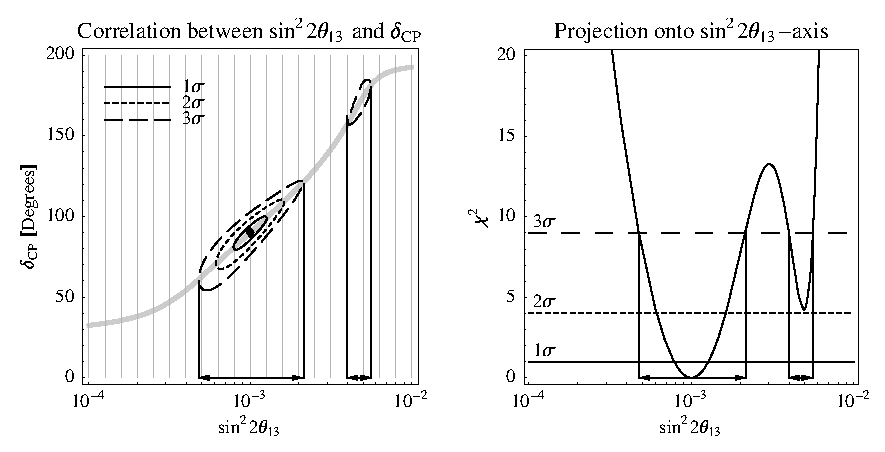
\includegraphics[width=16cm]{projex}
\end{center}
\mycaption{\label{fig:projex} Left plot: The correlation between $\stheta$ and $\deltacp$ as calculated in the example on page~\pageref{ex:corrth13dcp}, but for 1 d.o.f. only. Right plot: The $\chi^2$-value of the projection onto the $\stheta$-axis as function of $\stheta$. The projection onto the  $\stheta$-axis is obtained by finding the minimum $\chi^2$-value for each fixed value of $\stheta$ in the left-hand plot, \ie, along the gray vertical lines. The thick gray curve marks the position of these minima in the left-hand plot. The arrows mark the obtained fit ranges for $\stheta$ at the $3 \sigma$ confidence level (1 d.o.f.), \ie , the precision of $\stheta$.}
\end{figure}

The projection onto the $\stheta$- (or $\deltacp$-) axis is performed by fixing $\stheta$ (or $\deltacp$) and minimizing the $\chi^2$-function over all free fit parameters and the matter densities. We illustrate this method at the example of the projection of the two-dimensional manifold in the $\stheta$-$\deltacp$-plane onto the $\stheta$-axis in \figu{projex}. In this figure, the left-hand plot shows the correlation in the $\stheta$-$\deltacp$-plane computed with {\tt Chi} or {\tt SingleChi}. The right-hand plot shows the projection of this two-dimensional manifold onto the $\stheta$ axis by minimizing $\chi^2$ over $\deltacp$. In this simple example, the minimization is done along the vertical gray lines in the left hand plot. The obtained minima are located on the thick gray curve, which means the the right-hand plot represents the $\chi^2$-value along this curve. In fact, one can easily see that one obtains the correct projected $3 \sigma$ errors in this example (\cf, arrows). This figure illustrates the projection of a two-parameter correlation. In general, the full $n$-parameter correlation is treated similarly by the simultaneous (local) minimization over all free fit parameters. The example on page~\pageref{ex:corrproj} demonstrates how one can obtain \figu{projex} (right) with keeping all parameters but $\deltacp$ fixed, as well as how one can inlcude the full $n$-parameter correlation with external input. It also demonstrates how these two compare to each other.

One mentioned disadvantage of the local minimizer is the possibility to end up in a local minimum. Usually it works very well to start the minimizer close to the best-fit values. In the example in \figu{projex}, the minimizer is always started at $\deltacp=90^\circ$ and finds its way to the appropriate minimum. In some cases, however, the topology may be more difficult and the true minimum is not correctly found. A strong indication for such a situation are discontinuities in the projected $\chi^2$-function, where the minimizer jumps from one minimum to the other. In such a case, the starting point of the minimizer has to be adjusted to help it find the true minimum. In other cases, the convergence of the minimizer may be infinitively small. Then it usually helps to start the minimizer somewhat off the best-fit values. The following functions are the simplest minimizers provided by \GLOBES :
\begin{function}
\GLB{ChiTheta}$( \theta_{13}, \, \{ \theta_{12}, \, \theta_{23}, \, \deltacp , \, \sdm , \, \ldm, \, \hat{\rho_1}, \,  \hdots ,  \,\hat{\rho_n} \})$ returns the projection onto the $\theta_{13}$-axis for all experiments. The parameters are the fixed value of $\theta_{13}$ and the starting point of the minimizer including all starting values for the matter density scaling factors (without $\theta_{13}$, which is fixed). The return value is a list $\{ \chi^2, \, \theta_{12}, \, \theta_{23}, \, \deltacp , \, \sdm , \, \ldm, \, \hat{\rho_1}, \, \hdots , \, \hat{\rho_n} , \, N_{\mathrm{Iter}} \}$ with the minimum $\chi^2$ found, the coordinates of the local minimum (without $\theta_{13}$), and the number of iterations $N_{\mathrm{Iter}}$ used by the minimizer (number of function calls of {\tt Chi}).
\end{function}
\begin{function}
\GLB{SingleChiTheta}$( \theta_{13}, \, \{ \theta_{12}, \, \theta_{23}, \, \deltacp , \, \sdm , \, \ldm,  \, \hat{\rho}_{N_{\mathrm{exp}}} \}, \, N_{\mathrm{exp}})$ works similar to {\tt ChiTheta}, but only for one of the loaded experiments $N_{\mathrm{exp}}$. It returns the list $\{ \chi^2, \, \theta_{12}, \,  \theta_{23}, \, \deltacp , \, \sdm , \, \ldm, \, \hat{\rho}_{N_{\mathrm{exp}}} , \, N_{\mathrm{Iter}} \}$.
\end{function}
\begin{function}
\GLB{ChiDelta}$( \deltacp, \, \{ \theta_{12}, \, \theta_{13}, \, \theta_{23}, \, \sdm , \, \ldm, \, \hat{\rho_1}, \,  \hdots ,  \,\hat{\rho_n} \})$ returns the projection onto the $\deltacp$-axis for all experiments. The parameters are the fixed value of $\deltacp$ and the starting point of the minimizer including all starting values for the matter density scaling factors (without $\deltacp$, which is fixed). The return value is a list $\{ \chi^2, \, \theta_{12}, \, \theta_{13}, \, \theta_{23}, \, \sdm , \, \ldm, \, \hat{\rho_1}, \, \hdots , \, \hat{\rho_n} , \, N_{\mathrm{Iter}} \}$ with the minimum $\chi^2$ found, the coordinates of the local minimum (without $\deltacp$), and the number of iterations $N_{\mathrm{Iter}}$ used by the minimizer (number of function calls of {\tt Chi}).
\end{function}
\begin{function}
\GLB{SingleChiDelta}$( \deltacp, \, \{ \theta_{12}, \, \theta_{13}, \, \theta_{23}, \, \sdm , \, \ldm, \,  \hat{\rho}_{N_{\mathrm{exp}}} \}, \, N_{\mathrm{exp}})$ works similar to {\tt ChiDelta}, but only for one of the loaded experiments $N_{\mathrm{exp}}$. It returns the list $\{ \chi^2, \, \theta_{12}, \,  \theta_{13}, \,  \theta_{23}, \, \sdm , \, \ldm, \, \hat{\rho}_{N_{\mathrm{exp}}} , \, N_{\mathrm{Iter}} \}$.
\end{function}
All of these function have the same parameter structure: The fixed parameter is not transferred in the list, but as a the first separate parameter. The number of matter density scaling factors corresponds to the number of experiments used, since each experiment may face other matter density conditions. Note that before any of these function calls, {\tt SetStartingValues} and {\tt SetInputErrors} have to be used at least once. In addition, note that the resulting $\chi^2$ of {\tt ChiTheta} (or {\tt ChiDelta}) is not the sum of the $\chi^2$-values over all {\tt Single}-functions of all experiments anymore. This has two reasons: First, the topology of the fit manifold is altered by the addition of $\chi^2$-values of different experiments. Thus, after the minimization, the position of the minimum can be different to the ones of the individual experiments. Second, the priors for the external knowledge on the parameters are only added once -- independent of the number of experiments. A simple application of {\tt ChiTheta} can be found in the example on page~\pageref{ex:corrproj}. 

The return values of these functions do not only contain the minimum $\chi^2$-value found, but also the position of the minimum. This information can often be valuable, since one can often quickly locate irregularities: If one of the parameters is far off the best-fit value, the minimzer may have ended up in a local unwanted minimum. For instance, a negative value of $\ldm$ (with a positive best-fit value) indicates that the minimizer ended up in the opposite-sign solution. Another possibility is that the experiment may not be able to determine the measured parameter at all without external knowledge about the parameter far off its best-fit value. In both cases, an externally imposed precision on the run-off parameter can help to solve the problem. 

\section[Projection onto any hyperplane]{Projection onto any  hyperplane}
\index{Projection onto hyperplane}

In general, one can show the measurement result in any $k$-dimensional hyperplane, where $k$ is smaller than the dimension of the parameter space $n$, and thus the dimension of the fit manifold. In this case, $k$ parameters are fixed and $n-k$ parameters are minimized over. One such example is the projection of the fit manifold onto the $\stheta$-$\deltacp$-plane, \ie, $k=2$ here. This projection can be performed with the following functions:
\begin{function}
\GLB{ChiThetaDelta}$(\theta_{13}, \, \deltacp, \, \{ \theta_{12}, \, \theta_{23},  \, \sdm , \, \ldm, \,   \hat{\rho_1}, ... , \hat{\rho_n} \})$ returns the list  $\{ \chi^2, \, \theta_{12}, \, \theta_{23}, \, \sdm , \, \ldm,  \, \hat{\rho_1}, \, \hdots , \, \hat{\rho_n} , \, N_{\mathrm{Iter}} \}$ for the projection into the $\theta_{13}$-$\deltacp$-plane for all experiments.
\end{function}
\begin{function}
\GLB{SingleChiThetaDelta}$( \theta_{13}, \, \deltacp, \, \{ \theta_{12}, \, \theta_{23}, \, \sdm , \, \ldm, \,   \hat{\rho}_{N_{\mathrm{exp}}} \}, \, N_{\mathrm{exp}})$ returns the list $\{ \chi^2, \, \theta_{12}, \,   \theta_{23},  \, \sdm , \, \ldm, \, \hat{\rho}_{N_{\mathrm{exp}}} ,  \, N_{\mathrm{Iter}} \}$ for the projection into the $\theta_{13}$-$\deltacp$-plane for one experiment $N_{\mathrm{exp}}$.
\end{function}
These functions work analogously to the ones in the last section. They can, for example, be used to obtain a figure similar to \figu{projex}, left. However, the result would not be a two-dimensional cut through the fit-manifold, but a two-dimensional projection. Though the running time for one call of these functions is somewhat shorter than the one for the $\stheta$- or $\deltacp$-projections, one has to compute a two-dimensional array for such a figure (instead of a one-dimensional list). Therefore, the overall computational effort is much higher.

In principle, one can also use three- or more-dimensional projections. In addition, one may want to use any other set of parameters for single- or two-parameter projections. The functions {\tt ChiNP} and {\tt SingleChiNP} are designed for this purpose:

FUNCTIONS TO BE DEFINED. (WORK IN PROGRESS).

\chapter{Finding degenerate solutions}
\index{Degenerate solutions}

In the last chapter, we introduced the projection of any set of $k$ parameter onto any $n-k$ dimensional hyperplane, which was done by the minimization over the $k$ free fit parameters. Similarly, one can minimize over {\em all} $n$ parameters to find the local minimum close to any starting point. This approach is very useful for the exact numerical location of a degenerate if its approximate position is known. For the determination of the approximate positon, one can use analytical approaches, such as in \Refs~TO BE ENTERED, or an educated guess. 
Though the usage of the all-parameter minimizers is quite simple, one should keep in mind that they are local minimizers. Therefore, one may need a very sophisticated application software to actually find all degenerate solutions.

\example{Finding the $\mathrm{sgn}(\ldm)$-degeneracy}{
\label{ex:sgndeg}

In many cases, one can find the exact position of the $\mathrm{sgn}(\ldm)$-degeneracy with \GLB{glbChiAll}, where one starts 
the local minimizer at the suspected position 
and let it converge into the minimum.  The following code excerpt  corresponds to finding the degenerate solution for the example on
  page~\pageref{ex:corrth13dcp}, and it is from {\tt example3.c}: 
\begin{quote}
{\tt
{\footnotesize
  /* Set starting vales to suspected position at opposite sign of ldm */ \\
  \mbox{glbDefineParams(starting\_values,theta12,theta13,theta23,deltacp,sdm,-ldm);} \\
  \\
  /* Set input errors for external input, where some information on ldm \\
   \hspace*{0.5cm} is imposed in order to avoid falling into the right-sign solution */ \\
  glbDefineParams(input\_errors,theta12*0.1,10,10,10,sdm*0.1,ldm/3); \\ 
  glbSetDensityParams(input\_errors,0.05,GLB\_ALL); \\
  \\
  glbSetStartingValues(starting\_values); \\
  glbSetInputErrors(input\_errors); \\
  \\
  /* Localize degenerate solution by minimzation over all parameters */ \\
  double CL=glbChiAll(starting\_values,deg\_pos,GLB\_ALL); \\
   \\
  \mbox{/* Now: CL is the chi2 of the deg.~solution and deg\_pos the position */} 
}}
\end{quote}

Using {\tt ent\_pos} to obtain a section of the degeneracy in the
$\stheta$-$\deltacp$-plane (\cf, {\tt example3.c}), one can plot it as a contour plot in addition to the original solution (2 d.o.f., gray curves):
\begin{center}
\colorbox{white}{\includegraphics[width=7.5cm]{correntex}}
\end{center}

}

\index{All-parameter minimization}
The functions to perform the all-parameter minimization are {\tt ChiAll} and {\tt SingleChiAll}:
\begin{function}
\GLB{ChiAll}$(\{ \theta_{13}, \, \theta_{12}, \, \theta_{23}, \, \deltacp , \, \sdm , \, \ldm,  \, \hat{\rho_1}, \, \hdots , \, \hat{\rho_n} \})$ finds the local minimum close to the given starting point (list) for all initialized experiments. It returns the list  $\{ \chi^2, \, \theta_{13}, \, \theta_{12}, \, \theta_{23}, \, \deltacp , \, \sdm , \,  \ldm,  \, \hat{\rho_1}, \, \hdots , \hat{\rho_n} , \, N_{\mathrm{Iter}} \}$ with the minimum $\chi^2$-value, the actual position of the local minimum, and the number of iterations $N_{\mathrm{Iter}}$ used.
\end{function}
\begin{function}
\GLB{SingleChiAll}$( \{ \theta_{13}, \, \theta_{12}, \, \theta_{23}, \, \deltacp , \, \sdm , \, \ldm, \,   \hat{\rho}_{N_{\mathrm{exp}}} \}, \, \, N_{\mathrm{exp}})$ finds the local minimum close to the given starting point (list) for the experiment $N_{\mathrm{exp}}$ only. It returns the list
 $\{ \chi^2, \, \theta_{13}, \, \theta_{12}, \, \theta_{23}, \, \deltacp , \, \sdm , \, \ldm, \, \hat{\rho}_{N_{\mathrm{exp}}} ,  \, N_{\mathrm{Iter}} \}$ with the minimum $\chi^2$-value, the actual position of the local minimum, and the number of iterations $N_{\mathrm{Iter}}$ used.
\end{function}
%
Both functions take the suspected position of the local minimum and return its true position. The application of  {\tt SingleChiAll} can be especially usefull for many different experiments evaluated simultaneously: It turns out to be useful to find the positions of the degeneracies for the individual experiments first, and then test all of these with the combination of all experiments in order not to miss a degenerate solution. The example on page~\pageref{ex:sgndeg} illustrates how to locate the $\mathrm{sgn}(\ldm)$-degeneracy and show the corresponding degenerate solution in the $\stheta$-$\deltacp$-plane together with the original solution.
In this case, the position of the degeneracy can be easily guessed to be at the best-fit parameter values but the $\ldm$ inverted. The minimizer then runs off the plane of the best-fit parameters into the local minimum. It is very important to take into account the position of the degeneracy off this plane, since the actual $\chi^2$ in the minimum is certainly lower than on the plane of the best-fit parameter values. Thus, the degeneracy may not even appear at the chosen confidence level on the plane, but it does appear at the true minimum. The two cuts\footnote{The discussed figure on page~\pageref{ex:sgndeg} is produced by  {\tt Chi} and thus only represents a cut through the fit manifold. For the projection including correlations, one may rather want to use {\tt ChiThetaDelta}.} through the fit manifold shown in the figure on page~\pageref{ex:sgndeg} therefore do not have the same oscillation parameter values (except from the ones shown in the figure). 

In practice, a number of tricks can be useful for the treatment of degenerate solutions:
\begin{description}
\item[Minimum $\boldsymbol{\chi^2}$ larger than threshold.] If a located degeneracy has a minimum $\chi^2$ larger than the corresponding confidence level threshold for the discussed quantity of interest, the degeneracy can be immediately ignored. This saves a lot of computation time.
\item[Locating degeneracies with more complicated topologies.] For more complicated topologies, such as for neutrino factories, it is often useful to use multi-step location procedures or analytical knowledge. For example, for a numerical procedure, one may first of all switch off the systematics and keep $\stheta$ or $\deltacp$ fixed, \ie, use {\tt SingleChiTheta} or {\tt SingleChiDelta}, where $\stheta$ or $\deltacp$ is fixed to the best-fit value. The result can then be used as a starting point for {\tt SingleChiAll} with the systematics switched on again. In addition to switching off the systematics, it can be useful to reduce the input errors during the first steps in order to make the minimizer not to run away too much from the true solution.
\item[Finding degeneracies with multiple experiments.] For multiple experiments, the degeneracies should be located for each of the individual experiments first. Then, all of the found degeneracies below the threshold can be tested for the combination of experiments.  
\end{description}
Finally, note that any degenerate solution below the confidence level threshold which can not be located makes the result appear better than it actually is. Thus, one should be careful with the determination of the degenerate solutions.

\chapter{Obtaining low-level information}

\bi
\item
 Obtaining rate vectors
\item
 Obtaining fluxes/cross sections etc.
\item
 ``Check''-functions
\ei

\example{The impact of systematics, correlations, and degeneracies}{
\label{ex:corrproj}
\index{Bar charts}
\index{Systematics on/off}
Here it is demonstrated how one can successively include systematics, correlations, and degeneracies at the example of the $\stheta$-sensitivity limit.
An important part of this example is how two switch the systematics off,
\ie, how to obtain the sensitivity limit from statistics only. Since
this example is very advanced, we only show the respective function of the code:
\begin{quote}
{\tt 
/* Calculate chi2 with statistics only */ \\
double CalcNoSystematics(double theldm,double thex) \\
\{ \\
\hspace*{0.5cm} /* Switch systematics off for all exps and all rules */ \\
\hspace*{0.5cm} glbSwitchSystematics(GLB\_ALL,GLB\_ALL,GLB\_OFF); \\
\\
\hspace*{0.5cm} /* Calculate Chi2-list as if systematics were on */ \\
\hspace*{0.5cm} double res=CalcSystematics(theldm,thex); \\
\\
\hspace*{0.5cm} /* Switch systematics on for all exps and all rules */ \\
\hspace*{0.5cm} glbSwitchSystematics(GLB\_ALL,GLB\_ALL,GLB\_ON); \\
\\
\hspace*{0.5cm} return res; \\
\} \\
}
\end{quote}

\vspace*{-0.5cm}

The complete code can be found as {\tt example4.c} with the software,
which consists of many of the applications from the earlier examples.
In addition, it uses a little trick: It avoids falling into the wrong
 solution with {\tt glbChiTheta}
by using the fit value of $\deltacp$ from the step before as prediction
of the position of the current calculation.

The returned lists of data from thie example represent $\chi^2$ 
as function of the fit value of $\stheta$. The intersections of these
curves with the line $\chi^2 = 9$ give the $\stheta$ sensitivity
limits at the $3 \sigma$ confidence level, where we do not include the
 $\mathrm{sgn}(\ldm)$- and $(\deltacp,\theta_{13})$-degeneracies in the sensitivity limit with correlations only (green bar):
\begin{center}
\colorbox{white}{\includegraphics[width=6.5cm]{barsex}}
\end{center}
}

\chapter{Changing experiment parameters at running time}

\bi
\item
 Baseline, Target mass, Source power, running time
\item
 Matter density profile
\item
 Systematics
\item
 Threshold function, efficiencies etc.
\ei